\documentclass{bmvc2k}

%% Enter your paper number here for the review copy
\bmvcreviewcopy{64}

\title{Benchmarking Text Detection in Video}

% Enter the paper's authors in order
% \addauthor{Name}{email/homepage}{INSTITUTION_CODE}
\addauthor{Phuc Xuan Nguyen}{http://www.vision.inst.ac.uk/~ss}{1}
\addauthor{Kai Wang}{http://www.vision.inst.ac.uk/~pp}{1}
\addauthor{Serge Belongie}{colin@collaborators.com}{2}

% Enter the institutions
% \addinstitution{Name\\Address}
\addinstitution{
 The Vision Institute\\
 University of Borsetshire\\
 Wimbleham, UK
}
\addinstitution{
 Collaborators, Inc.\\
 123 Park Avenue,\\
 New York, USA
}

\runninghead{Student, Prof, Collaborator}{BMVC Author Guidelines}

% Any macro definitions you would like to include
% These are not defined in the style file, because they don't begin
% with \bmva, so they might conflict with the user's own macros.
% The \bmvaOneDot macro adds a full stop unless there is one in the
% text already.
\def\eg{\emph{e.g}\bmvaOneDot}
\def\Eg{\emph{E.g}\bmvaOneDot}
\def\etal{\emph{et al}\bmvaOneDot}

%------------------------------------------------------------------------- 
% Document starts here
\begin{document}

\maketitle

\begin{abstract}
Text detection has been an interesting and challenging problem in computer vision, with many important real-life applications. While there are many publicly available datasets in the static image domain, the same attention has not been observed in the video domain. To establish a standard benchmark in video text detection, we create a UCSD Video Text Dataset. The dataset contains unconstrained videos extracted from online video platform. The videos are fully annotated with the locations of text regions, which have a wide variety of appearance. We also benchmarking existing image-domain text detection techniques, combined with technique that use temporal features to boost performance. By analyzing the results, we draw conclusions and suggestions for future works in text detection in video domain.

\end{abstract}

%------------------------------------------------------------------------- 
\section{Introduction}
\label{sec:intro}
Whereas Optical Character Recognition (OCR) technology for scanned, printed pages of text has seen great advances in recent decades, such technology has been slow to translate into the diverse and challenging domain of video. Beyond improving the indexability of video content in general, a solution to this problem is certain to provide compelling opportunities for context sensitive advertising and marketing for broadcast TV.

Detecting text in unconstrained images and videos are a challenging problem

There is an increasing interests in text detection and text recognition. Need to mention OCR, and how it fails in the general situation.

Mention the fact that there are a lot of videos traffic going on.

Segment into the application of text detection in videos: disability assistance, video indexing, video categories, navigations

\paragraph{Contributions}

\begin{enumerate}

\item We introduce the UCSD Video Text Dataset, containing a large amount of annotated videos

\item We benchmark different approaches toward text detection.

\item Analysis
\end{enumerate}

We introduce the UCSD Video Text Detection Data and describe its statistics in Sec. 2.
\section{Related Methods and Datasets}
There are many annotated datasets publicly available for text detection and recognition domain. The Street View Text(SVT) dataset \cite{WangBB11} composes of images harvest from Google Street View. Most text apperances come from business and street signs. The dataset contains word-level annotations and mainly used for lexicon-driven word recognition.

ICDAR provides dataset. ICDAR has become a standard dataset to compare detection results.

Chars74K offers the character images from both

Table ? offer the summary of the available dataset in the static domain.

Even though there have been many works in the literature in text detection in domain, a publicly available dataset has not surfaced during our literature review. Most research groups created their own datasets and followed different annotation processes. Furthermore, these datasets are not released to the public. Hence, there is no clear answer in which approach is best for text detection in video.

\section{Dataset}
\subsection{Collection Process}

We break our annotation process into 3 phases: collection, filtering, and annotation.
\paragraph{Phase 0 - Collection} We crawl YouTube using videos feeds returning from query terms, such as, "sports", "music", "politics", etc. From each of the feed video, we download its related videos and repeat. We only download videos that have HD 720p quality.

\paragraph{Phase 1 - Filtering} As we have no filtering in phase 1, there are many videos, or parts of videos, that do not have text content. We want to filter out the majority of these non-text contents. First, we divide the original videos into 15-second segments. We then use Amazon Mechanical Turk to filter out these segments. We create Human Intelligence Tasks(HITs), in which the users are presented with a 15-second video segments and asked whether the video contains visible and readable text.

\paragraph{Phase 2 - Annotation} Ater phase 1, we have a database of 15-second segments are annotated as containing text. We are, however, interested in the exact location of text appearance on every frame. We use the VATIC tools(need citation) to help with the problem of video annotation. We instruct the users to draw the bounding boxes over the text region.

\section{Dataset Statistics}

Our dataset contains 500(need to update this number) 15-second video segments. Each video segment has either 24 or 30 frame per second. In total, we annotated 150000 frames for a total of 200000 bounding boxes of text region.

\paragraph{Type} The literature of text detection and recognition often divides text occurence into two types: overlay text and scene text. We define overlay text as those are edited into the video and scene text as those incidentally happened in the scene. Scene text is often harder to detect and recognize than overlay text. Out of all the bounding boxes, 30\% are scene texts. Figure ? shows examples of scene text and overlay text in the dataset.

\paragraph{Position} We accumulate the text region over the dataset and plot the resulting heat map. In Figure ?, we shows the expected locations of scene texts and overlay text in the dataset. As we can see, overlay texts usually appear in a more certain situation while scene text appears more randomly in the scene.

\paragraph{Scale} We aim for the datasets to contain a wide variety of scales Figure ? shows the distribution of percentage of the frames belongs to the text region.

\paragraph{Categories} We keep track of the category of each video to ensure a good distribution of categories. This helps reducing biases from video categories and vary the appearance of text in the dataset. Figure ? shows the distribution of video categories in the dataset.

\subsection{Training and Testing Data}
The video segments in our dataset comes from 250 original videos. We split the segments into the training set and testing set based on their original videos. The segments belong to the first 125 videos are in the training set and the other 125 videos are in the testing.

\section{Evaluation methodology}
In this paper, we are concerned with the location of region in the image. We use pixel-based performance metric to benchmark the approachs. <We need an explanation for it here>. We define hit and miss as followed: (equations here).

\section{Experiments}
\subsection{Text Detection}

\paragraph{HOG+SVM} An object detection pipeline using HOG features and a linear SVM as classifier has become a norm in the Computer Vision community. There has been many work in the text detection literature that involves the sliding window approach. We aim to evaluate this approach in the video text detection domain. In our implementation, we use Piotr Dollar's HOG implementation and liblinear for the linear SVM.

We sample positives data point from the ICDAR and SVT dataset. For each text patch, we scan a fixed size window to extract the positive example. Figure ? shows the example of positive patches in our dataset. We obtain the negative patch from randomly sampling from images from the FlickR dataset. We manually go through each image in this dataset to make sure that there is no obvious text apperance in the picture. We treat the Flickr dataset as a negative pool. From this pool, we also did many rounds of hard negative mining by selecting difficult patches in order to reduce false positives.

\paragraph{Combination of local detectors} Unlike the HOG+SVM approach, this approach does not train a single filter for text region, but rather builds 62 different character filters and combines these detections into one final detection. We use letter region segmented from ICDAR, Chars74K, and SVT(link to the right author) as positive data. For each character in the numericalphabets, we use that character and related characters as positive data and non-related characters to be initial negative data. We also perform many rounds of hard negative mining to reduce the number of false positives.

\paragraph{Stroke Width Transform} Stroke Width Transform\cite{swt10} is considered the leading technique in text detection. We benchmark an implementation from libccv(need link) with no modification to the original code.

\subsection{Temporal Smoothing} Unlike the static domain, we can exploit temporal features in the video domain and use these features to improve the performance. We base this technique on the observation that text appearance often persists more than N frames, and that false positives are often less persistent in the detection scheme.
\paragraph{Rule-based} Given a frame, we compute the intersections of every bounding box in the current frame with all the bounding boxes in the the previous and next N frames. Either all the previous or next intersections is more than 50\% of the area of the bounding box, we keep this bounding box, or else we discard it as false positive. More formally,

Let $b{}_{i}^{f}$ be the i-th bounding box in frame $f$, and the
intersection of this bounding box with all the bounding boxes in the
previous $N$-th frame is

\[
I(b_{i}^{f},N)=\begin{cases}
1 & b_{i}^{f}\bigcap(\bigcup_{j}b_{j}^{f-N})>0.5\\
0 & otherwise
\end{cases}
\]


We define a function $H$ that takes an $i$-th bounding box at frame
$f$, $b_{i}^{f}$, and returns either 1 for a true positive or 0
for a false positive. The function is defined as 
\[
H(b_{i}^{f})=\left(\sum_{j=1}^{N}I(b_{i}^{f},j)\ge\frac{N}{2}\right)\bigcup\left(\sum_{k=1}^{N}I(b_{i}^{f},-k)\ge\frac{N}{2}\right).
\]
\paragraph{Learning-based} Instead of setting a hard threshold on N and the percentage that current bounding box must overlap, we build a classifier to discriminate between false and true positives based on temporal features. We use the training set to train this classifer. We run each classifier described in the previous section against the training set to obtain a list of bounding boxes. We compare each of the obtained bounding boxes against the ground truth bounding box. We label a prediction as true positive if more than half of its area belongs to the ground truth region and false positive otherwise. We obtain a 8-dimension feature vector for each bounding box. For a bounding box at frame t, its feature vector is defined as
<formula here>

where abc is def. For bounding boxes near the begining and the end of the videos, we mirror the frame before or after it. This acts as giving more weights to the preceeding or proceeding frames when the information is absent. We use half of the training set to train this SVM and validate on the other half. We obtain the following weights from the linear SVM.


\begin{figure}
\begin{tabular}{ccc}
\bmvaHangBox{\fbox{\parbox{2.7cm}{~\\[2.8mm]
\rule{0pt}{1ex}\hspace{2.24mm}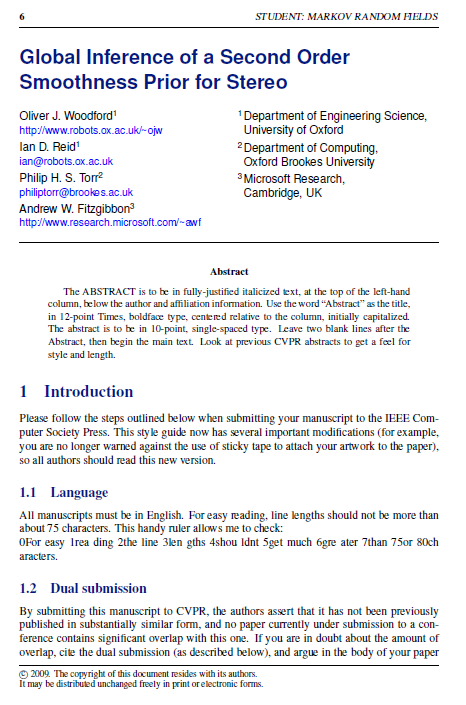
\includegraphics[width=2.33cm]{images/eg1_largeprint.png}\\[-0.1pt]}}}&
\bmvaHangBox{\fbox{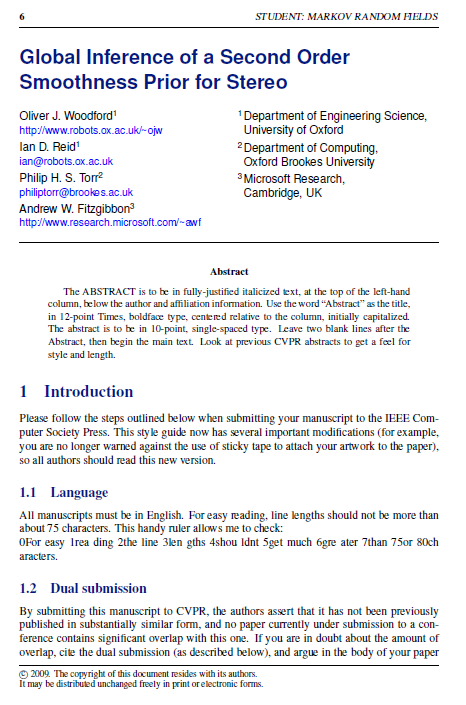
\includegraphics[width=2.8cm]{images/eg1_largeprint.png}}}&
\bmvaHangBox{\fbox{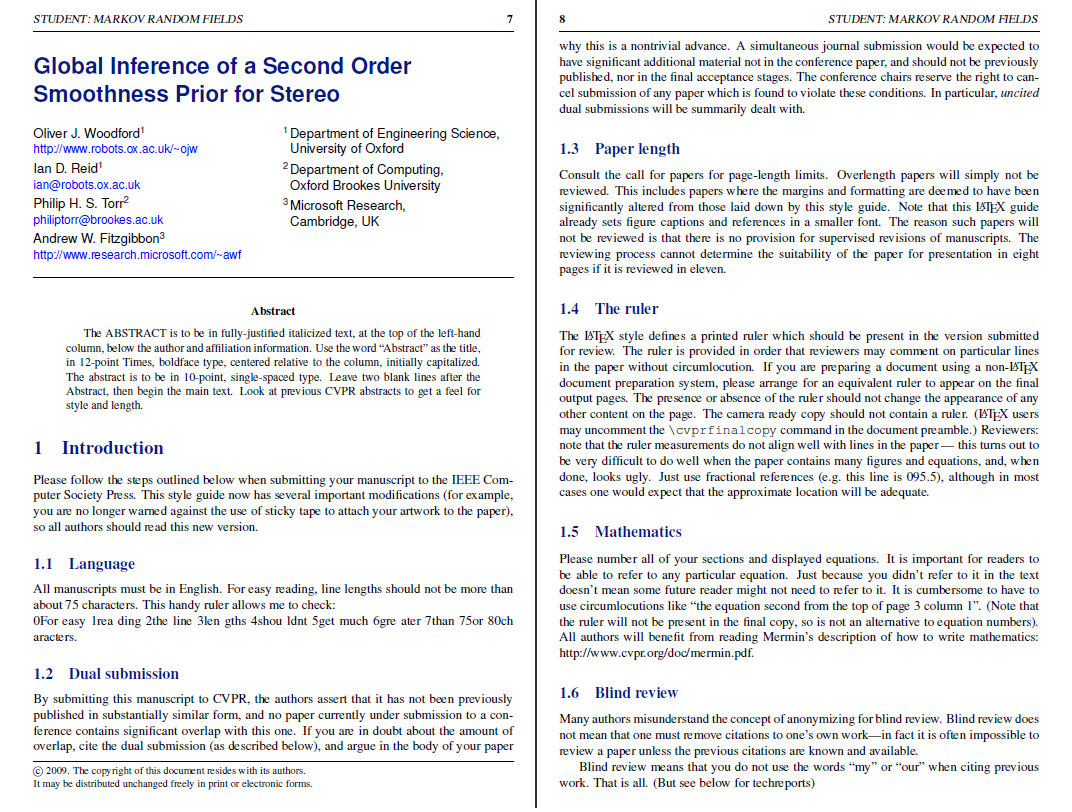
\includegraphics[width=5.6cm]{images/eg1_2up.png}}}\\
(a)&(b)&(c)
\end{tabular}
\caption{It is often a good idea for the first figure to attempt to
encapsulate the article, complementing the abstract.  This figure illustrates
the various print and on-screen layouts for which this paper format has
been optimized: (a) traditional BMVC print format; (b) on-screen
single-column format, or large-print paper; (c) full-screen two column, or
2-up printing. }
\label{fig:teaser}
\end{figure}

\begin{table}
\begin{center}
\begin{tabular}{|l|c|c|c|}
\hline
Method & Precision & Recall & f\\
\hline
HOG+SVM 			& -1 		& -1 & -1\\
HOG+SVM + T1 	& -1 		& -1 & -1\\
HOG+SVM + T2 	& -1 		& -1 & -1\\
LocalDet 		& -1 		& -1 & -1\\
LocalDet + T1 	& -1			& -1 & -1\\
LocalDet + T2 	& -1			& -1 & -1\\
SWT 				& 0.77 		& 0.74 & .75\\
SWT + T1 		& 0.83		& 0.73 & .77\\
SWT + T2 		& -1			& -1 & -1\\
\hline
\end{tabular}
\end{center}
\caption{Experiments results. T1 indicates that the results were temporally smoothed according to description in section ?, and T2 as in section ?. LocalDet stands for the combinations of local detectors.}
\end{table}

\subsection{Error Analysis}

\bibliography{egbib}
\end{document}
